\documentclass{beamer}
\mode<presentation> {
\usepackage{color}
\definecolor{bottomcolour}{rgb}{0.21,0.11,0.21}
\definecolor{middlecolour}{rgb}{0.21,0.11,0.21}
\setbeamercolor{structure}{fg=white}
\setbeamertemplate{frametitle}[default]%[center]
\setbeamercolor{normal text}{bg=black, fg=white}
\setbeamertemplate{background canvas}[vertical shading]
[bottom=bottomcolour, middle=middlecolour, top=black]
\setbeamertemplate{items}[circle]
\setbeamertemplate{navigation symbols}{} %no nav symbols
\setbeamercolor{block title}{use=structure,fg=white,bg=structure.fg!50!red!50!blue!100!green}
\setbeamercolor{block body}{parent=normal text,use=block title,bg=block title.bg!5!white!10!bg,fg=white}
\setbeamertemplate{navigation symbols}{}
\newcounter{moncompteur}
}
\usepackage{graphicx} 
\usepackage{booktabs} 
\usepackage[utf8]{inputenc}  
\usepackage{geometry}
%\usepackage[francais]{babel} 
\usepackage{eurosym}
\usepackage{verbatim}
\usepackage{ragged2e}
\justifying
%%%%%%%%%%%%%%%%%%%%%%%%%%%%%%%%%%%%%%%%%%%%%%%%%%%%%%%%%%%%%%%%
%% ccBeamer 0.1, 2007-07-02                                   %%
%% Written by Sebastian Pipping <webmaster@hartwork.org>      %%
%% ---------------------------------------------------------- %%
%% Licensed under Creative Commons Attribution-ShareAlike 3.0 %%
%% http://creativecommons.org/licenses/by-sa/3.0/             %%
%%%%%%%%%%%%%%%%%%%%%%%%%%%%%%%%%%%%%%%%%%%%%%%%%%%%%%%%%%%%%%%%


%% Images
\newcommand{\CcImageBy}[1]{%
	
\includegraphics[scale=#1]{creative_commons/cc_by_30.pdf}%
}
\newcommand{\CcImageCc}[1]{%
	
\includegraphics[scale=#1]{creative_commons/cc_cc_30.pdf}%
}
\newcommand{\CcImageDevNations}[1]{%
	
\includegraphics[scale=#1]{creative_commons/cc_dev_nations_30.pdf}%
}
\newcommand{\CcImageNc}[1]{%
	
\includegraphics[scale=#1]{creative_commons/cc_nc_30.pdf}%
}
\newcommand{\CcImageNd}[1]{%
	
\includegraphics[scale=#1]{creative_commons/cc_nd_30.pdf}%
}
\newcommand{\CcImagePd}[1]{%
	
\includegraphics[scale=#1]{creative_commons/cc_pd_30.pdf}%
}
\newcommand{\CcImageSa}[1]{%
	
\includegraphics[scale=#1]{creative_commons/cc_sa_30.pdf}%
}
\newcommand{\CcImageSampling}[1]{%
	
\includegraphics[scale=#1]{creative_commons/cc_sampling_30.pdf}%
}
\newcommand{\CcImageSamplingPlus}[1]{%
	
\includegraphics[scale=#1]{creative_commons/cc_sampling_plus_30.pdf}%
}


%% Groups
\newcommand{\CcGroupBy}[1]{% zoom
	\CcImageBy{#1}%
}
\newcommand{\CcGroupByNc}[2]{% zoom, gap
	\CcImageBy{#1}\hspace*{#2}\CcImageNc{#1}%
}
\newcommand{\CcGroupByNcNd}[2]{% zoom, gap
	\CcImageBy{#1}\hspace*{#2}\CcImageNc{#1}\hspace*{#2}\CcImageNd{#1}%
}
\newcommand{\CcGroupByNcSa}[2]{% zoom, gap
	\CcImageBy{#1}\hspace*{#2}\CcImageNc{#1}\hspace*{#2}\CcImageSa{#1}%
}
\newcommand{\CcGroupByNd}[2]{% zoom, gap
	\CcImageBy{#1}\hspace*{#2}\CcImageNd{#1}%
}
\newcommand{\CcGroupBySa}[2]{% zoom, gap
	\CcImageBy{#1}\hspace*{#2}\CcImageSa{#1}%
}
\newcommand{\CcGroupDevNations}[1]{% zoom
	\CcImageDevNations{#1}%
}
\newcommand{\CcGroupNcSampling}[2]{% zoom, gap
	\CcImageNc{#1}\hspace*{#2}\CcImageSampling{#1}%
}
\newcommand{\CcGroupPd}[1]{% zoom
	\CcImagePd{#1}%
}
\newcommand{\CcGroupSampling}[1]{% zoom
	\CcImageSampling{#1}%
}
\newcommand{\CcGroupSamplingPlus}[1]{% zoom
	\CcImageSamplingPlus{#1}%
}


%% Text
\newcommand{\CcLongnameBy}{Attribution}
\newcommand{\CcLongnameByNc}{Attribution-NonCommercial}
\newcommand{\CcLongnameByNcNd}{Attribution-NoDerivs}
\newcommand{\CcLongnameByNcSa}{Attribution-NonCommercial-ShareAlike}
\newcommand{\CcLongnameByNd}{Attribution-NoDerivs}
\newcommand{\CcLongnameBySa}{Attribution-ShareAlike}

\newcommand{\CcNote}[1]{% longname
	This work is licensed under the \textit{Creative Commons #1 3.0 License}.%
}

\title[Framasoft]{Framasoft - La Degooglisation} 
\author{Le Printemps de l'Entreprise - IUT de Vannes}
\begin{document}
%% Titlepage
\begin{frame}
	\titlepage
	\vfill
	\begin{center}
		\CcGroupByNcSa{0.83}{0.95ex}\\[2.5ex]
		{\tiny\CcNote{\CcLongnameByNcSa}}
		\vspace*{-2.5ex}
	\end{center}
\end{frame}


%-----------------------------------------------
\begin{frame}
\begin{center}
\Huge{Framasoft}
\\~\\

\includegraphics[scale=0.6]{./images/pingouinVolantRefait.jpg}
\end{center}
\end{frame}

%------------------------------------------------
\begin{frame}
\frametitle{Framasoft c'est quoi?}


\begin{block}{Présentation}
\justifying{
Association francophone de promotion et diffusion des logiciels libres. C'est aussi
\begin{itemize}
\item Un réseau dédié à la promotion du  libre  en général et du logiciel libre en particulier.
\item De nombreux services et projets innovants mis librement à disposition du grand public.
\item Une communauté de bénévoles soutenue par une association d’intérêt général.
\item Une invitation à bâtir ensemble un monde de partage et de coopération.
\end{itemize}
}
\end{block}
Plus de détail sur \url{http://www.framasoft.org}

\end{frame}
%-----------------------------------------------
\begin{frame}
\begin{center}
\Huge{Le logiciel libre}
\\~\\

\includegraphics[scale=0.8]{./images/linux.jpg}
\end{center}
\end{frame}

%-----------------------------------------------
\begin{frame}
\frametitle{Le logiciel libre}
\begin{block}{Les 4 libertés du logiciel libre}
\begin{itemize}
\justifying{
\item la liberté d'utiliser le logiciel ;
\item la liberté de copier le logiciel ;
\item la liberté d'étudier le logiciel ;
\item la liberté de modifier le logiciel et de redistribuer les versions modifiées.
}
\end{itemize}
\end{block}
\end{frame}

%-----------------------------------------------
\begin{frame}
\begin{center}
\Huge{Pour mieux comprendre,\\ une analogie  avec \\les recettes de cuisine...}
\end{center}
\end{frame}

%-----------------------------------------------
\begin{frame}
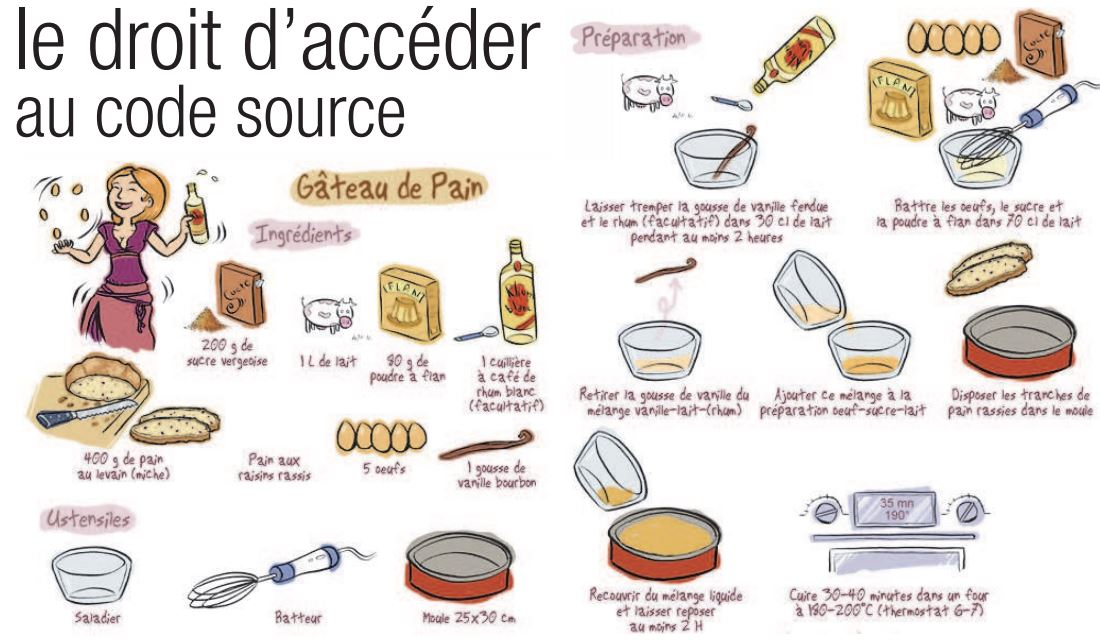
\includegraphics[scale=0.6] {./images/Cuisine01.jpg} 
\end{frame}
\begin{frame}
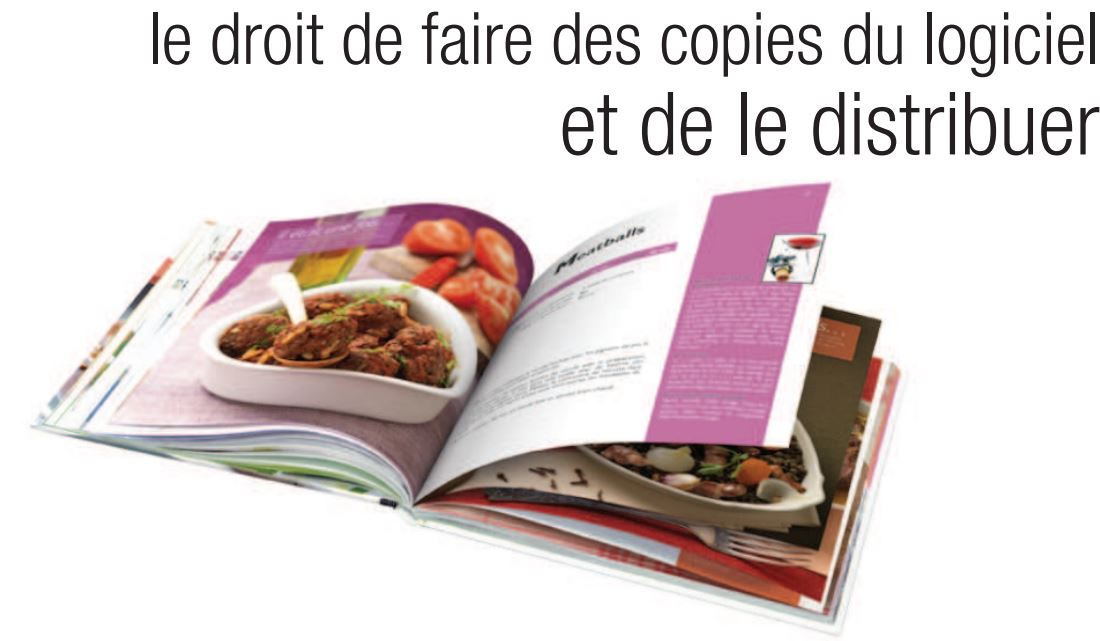
\includegraphics[scale=0.5] {./images/Cuisine02.jpg} 
\end{frame}
\begin{frame}
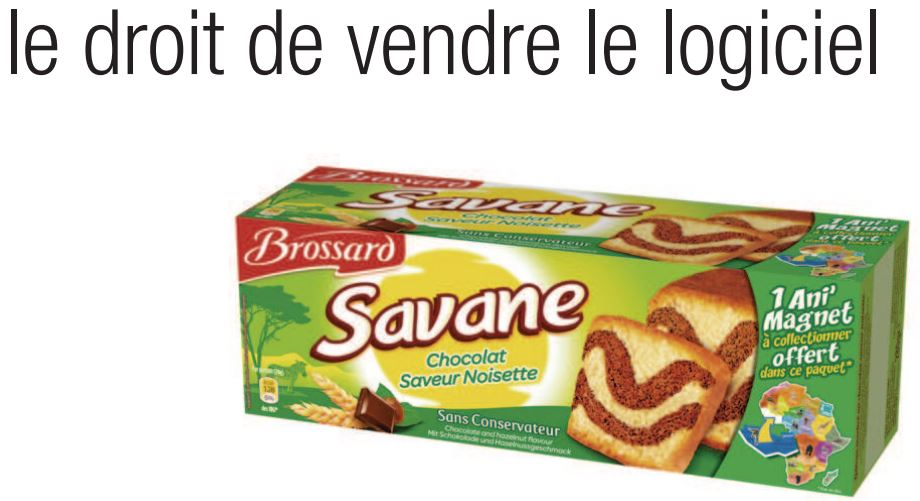
\includegraphics[scale=0.6] {./images/Cuisine03.jpg} 
\end{frame}
\begin{frame}
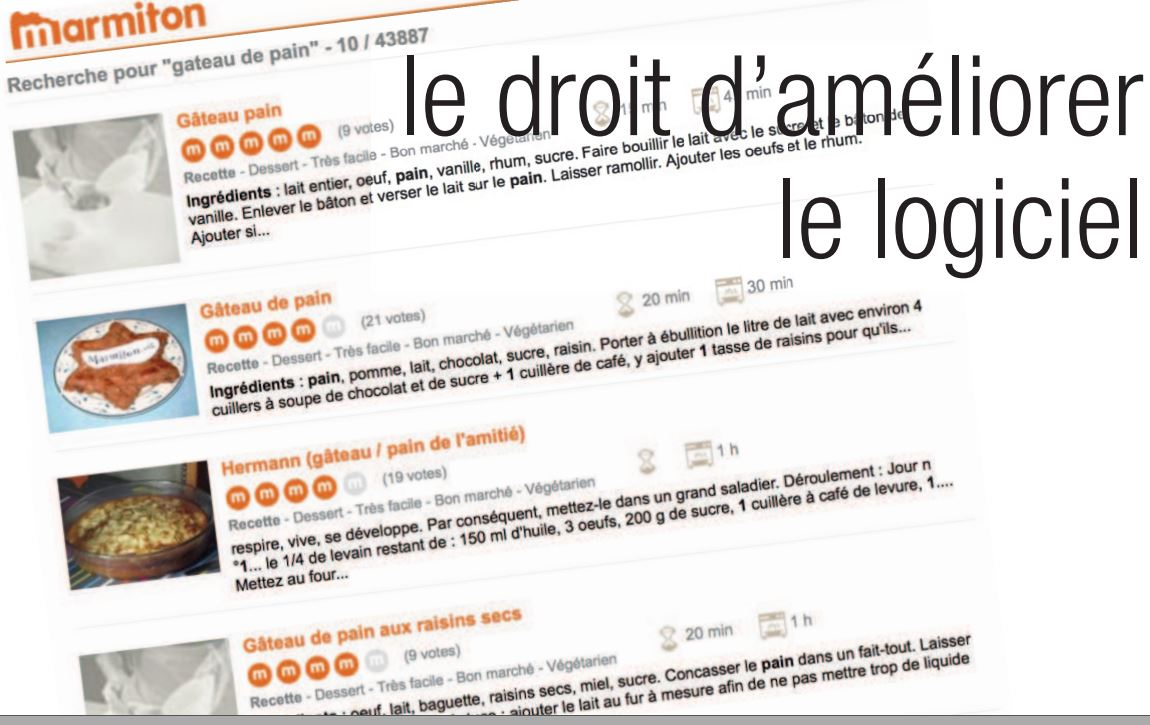
\includegraphics[scale=0.48] {./images/Cuisine04.jpg} 
\end{frame}

\begin{frame}
\frametitle{Quelques logos de logiciels libres connus}

\includegraphics[scale=0.5] {./images/Le_logiciel_libre.png} 
\end{frame}

%-----------------------------------------------
\begin{frame}
\begin{center}
\Huge{Les GAFAM}
\\~\\
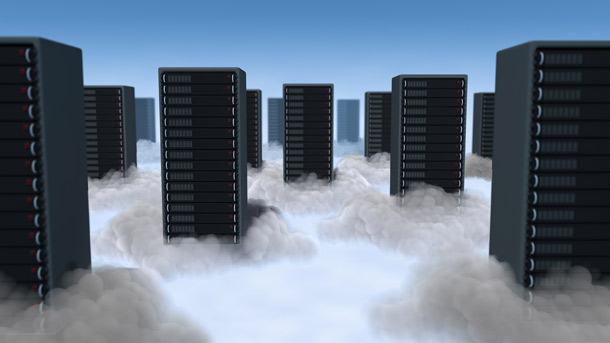
\includegraphics[scale=0.4]{./images/cloud_gafam.jpg}
\end{center}
\end{frame}

%------------------------------------------------
\begin{frame}
\frametitle{Les GAFAM}

\begin{block}{Les dangers}
\justifying{
Centralisation des données des utilisateurs chez quelques grands de l'Internet comme Google, Amazon, Facebook, Apple ou Microsoft (GAFAM)
\begin{itemize}
\item Espionnage
\item Vie privée
\item Centralisation
 \item Fermeture
\end{itemize}
\begin{center}
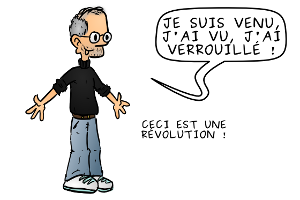
\includegraphics[scale=0.3]{./images/steve.png}\quad
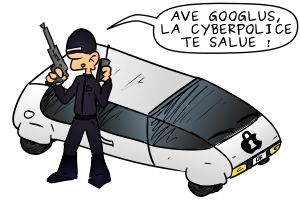
\includegraphics[scale=0.3]{./images/legion.png}
\end{center}
}
\end{block}
\end{frame}

%------------------------------------------------
\begin{frame}
\frametitle{Enjeux}

\begin{block}{Les enjeux}
\justifying{
\begin{itemize}
\item Concentration des acteurs d’Internet autour de sillos
\item Une centralisation nuisible (frein à l'innovation)
\item  Les utilisateurs de ces services derniers ne contrôlent plus leur vie numérique
\end{itemize}
\begin{center}

\includegraphics[scale=0.3]{./images/fight.png}
\end{center}
}
\end{block}
\end{frame}

%----------------------------------------------------------------------------------------
\begin{frame}
\Huge{\centerline{Framasoft et la dégooglisation}}
\begin{center}
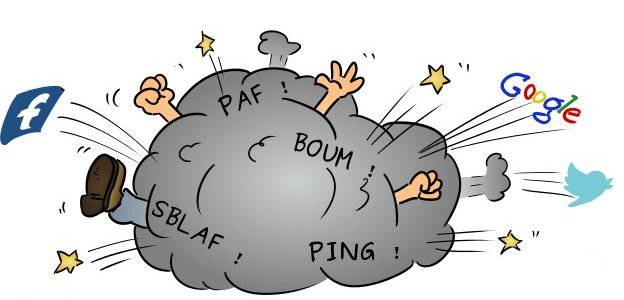
\includegraphics[scale=0.6]{./images/cloud.jpg}
\end{center}
\end{frame}

\begin{frame}
\begin{center}
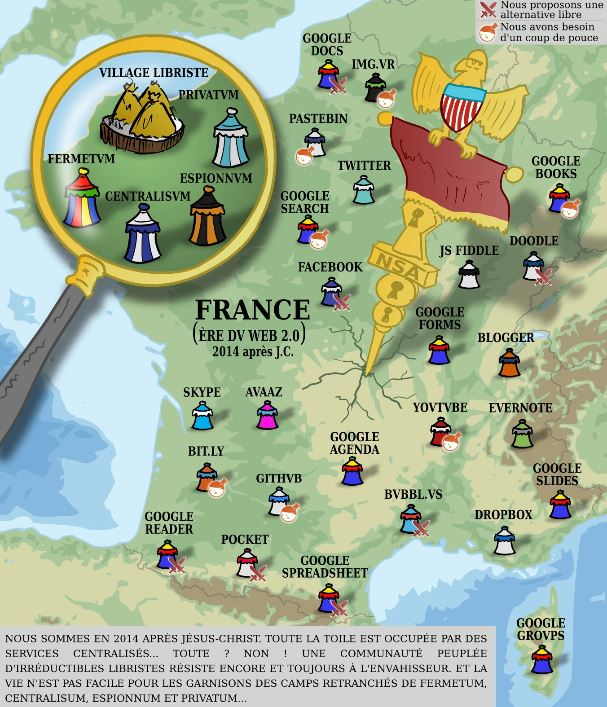
\includegraphics[scale=0.5]{./images/DegooglisonsInternet.jpg}
\end{center}
\end{frame}

%------------------------------------------------
\begin{frame}
\frametitle{Dégooglisons Internet}

\begin{block}{L'objectif}
\justifying{
Les logiciels libres, de par leur nature ouverte, sont les seuls à vraiment garantir le respect de votre vie privée.
\\~\\
Il faut donc installer, face à chaque service propriétaire, un service hébergé par les soins de Framasoft. 
\\~\\L’association s’inscrit dans un contexte d’ouverture en encourageant les projets qui participeront à cet effort d’émancipation des \emph{grands de l’Internet}.
}
\end{block}
Plus de détail sur \url{http://degooglisons-internet.org/}
\end{frame}

%------------------------------------------------
\begin{frame}
\frametitle{Les propositions de Framasoft}

\begin{block}{Ce que Framasoft propose}
\justifying{
Framasoft souhaite faire face à ces dangers menaçant nos vies numériques en proposant des services
\begin{itemize}
\item  libres,
\item éthiques, 
\item décentralisés 
\item et solidaires.
\end{itemize}
\begin{center}

\includegraphics[scale=0.3]{./images/potion.png}
\end{center}
}
\end{block}
\end{frame}

%------------------------------------------------
\begin{frame}
\frametitle{Concrètement, ce que fait Framasoft}

\begin{block}{Le projet \emph{Dégooglisons Internet} }
Consiste à proposer des services alternatifs face à un maximum de services que nous évaluons comme menaçants pour nos vies numériques.
\justifying{
\begin{itemize}
\item Des services qui sont libres, gratuits, ouverts à tous (dans la limite de nos capacités techniques et financières),
\item Promotion de l'auto-hébergement, 
\item Proposition d'alternatives.
\end{itemize}
}
\end{block}
Plus de détails sur \url{http://degooglisons-internet.org/}
\end{frame}

%----------------------------------------------------------------------------------------
\begin{frame}
\Huge{\centerline{Les services "cloud" de Framasoft}}
\begin{center}

\includegraphics[scale=0.6]{./images/Framacloud.jpg}
\end{center}
\end{frame}
%------------------------------------------------

\begin{frame}
\begin{center}
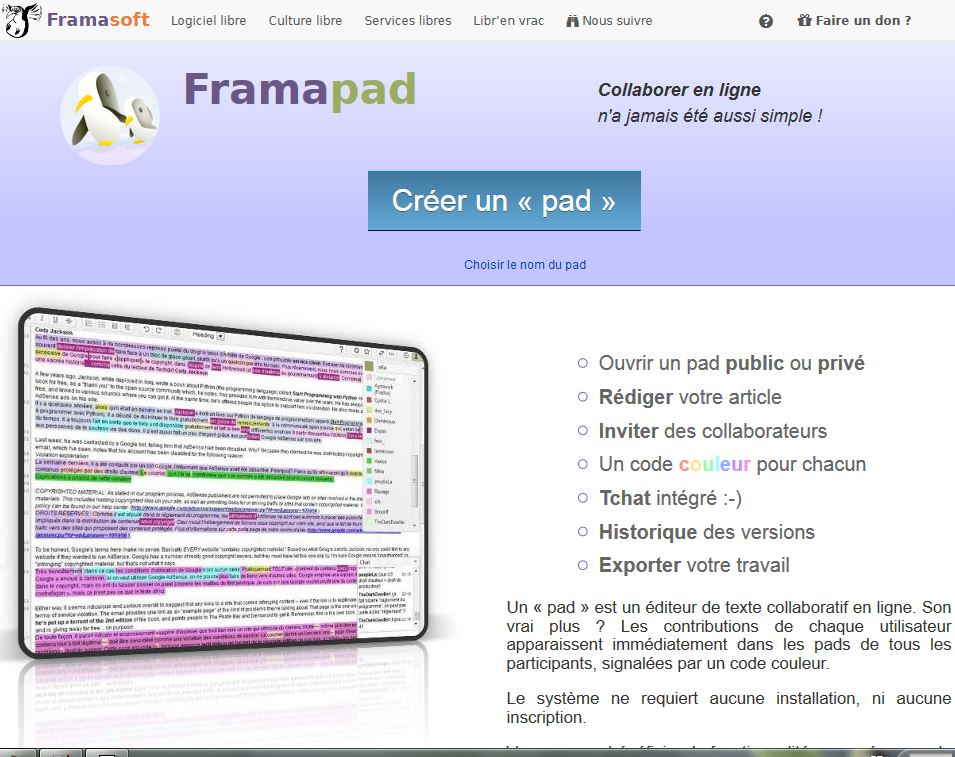
\includegraphics[scale=0.5]{./images/Framapad.jpg}
\end{center}
\end{frame}

\begin{frame}
\begin{center}
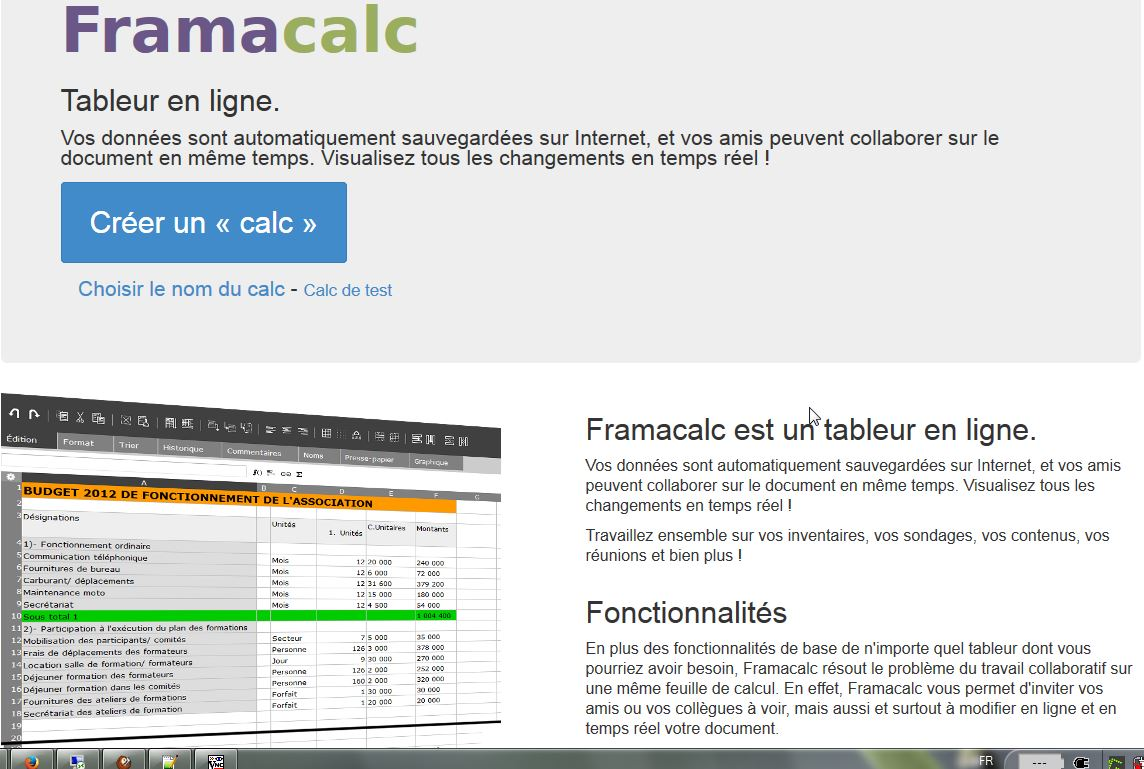
\includegraphics[scale=0.5]{./images/FramaCalc.jpg}
\end{center}
\end{frame}

\begin{frame}
\begin{center}
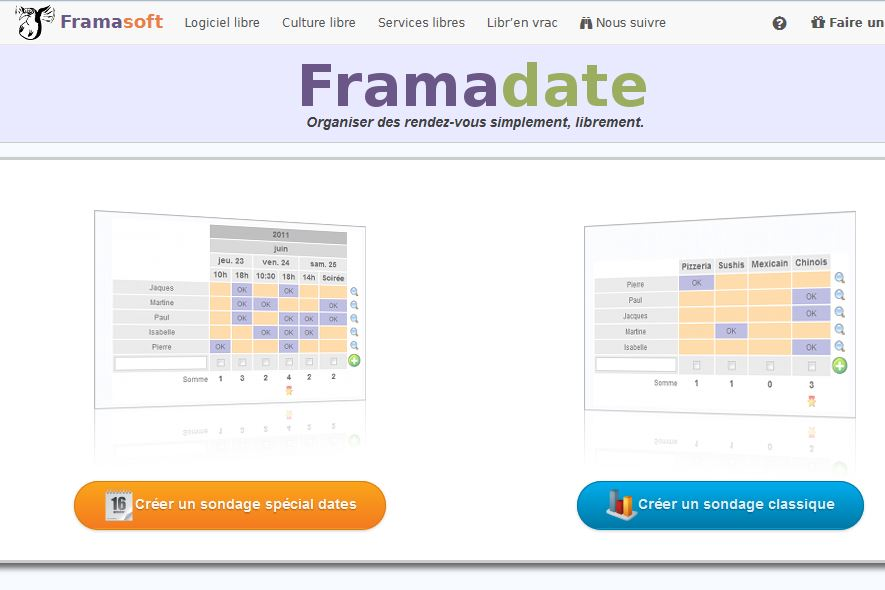
\includegraphics[scale=0.5]{./images/Framadate.jpg}
\end{center}
\end{frame}

\begin{frame}
\begin{center}
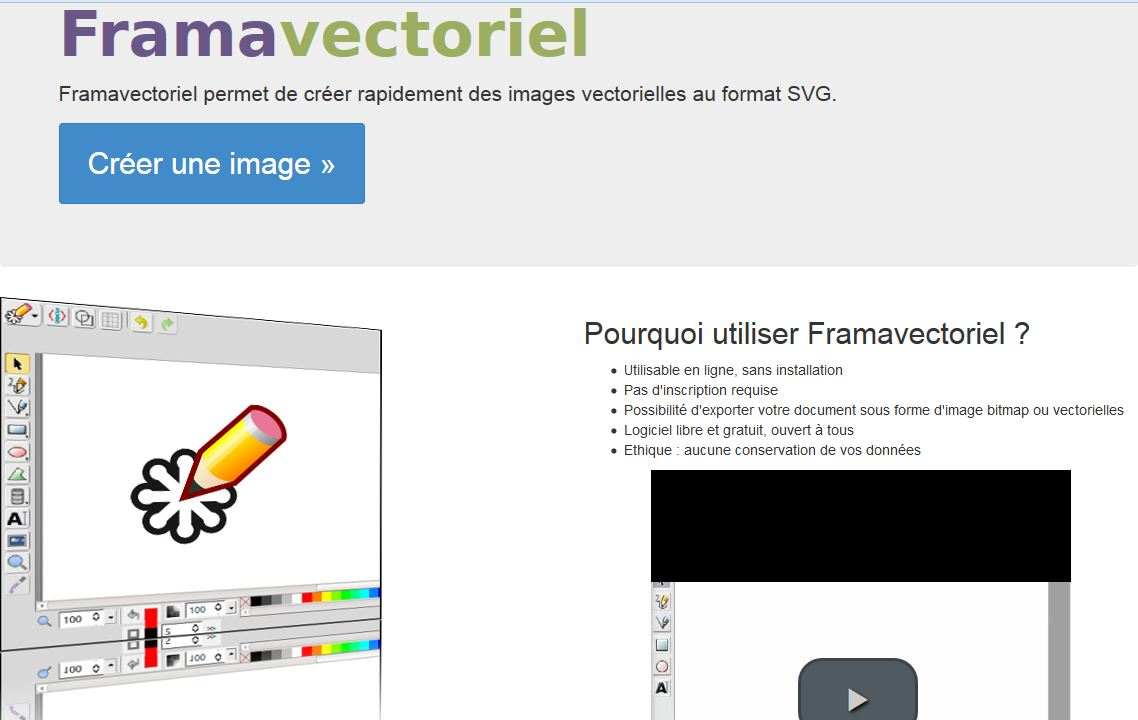
\includegraphics[scale=0.5]{./images/Framavectoriel.jpg}
\end{center}
\end{frame}

\begin{frame}
\begin{center}
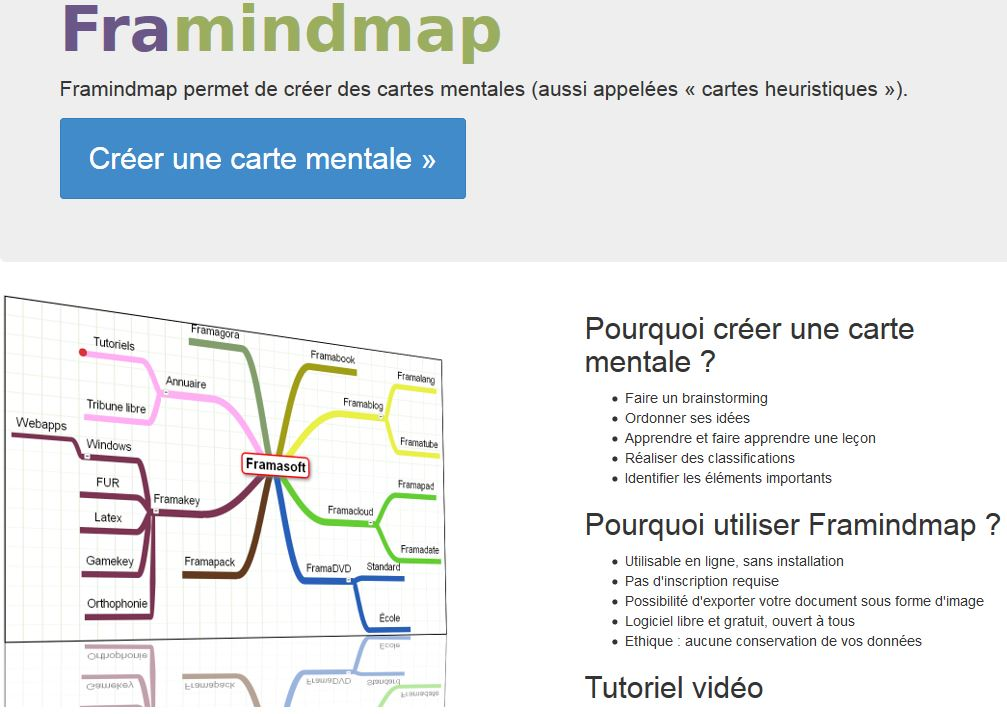
\includegraphics[scale=0.5]{./images/Framindmap.jpg}
\end{center}
\end{frame}

\begin{frame}
\begin{center}
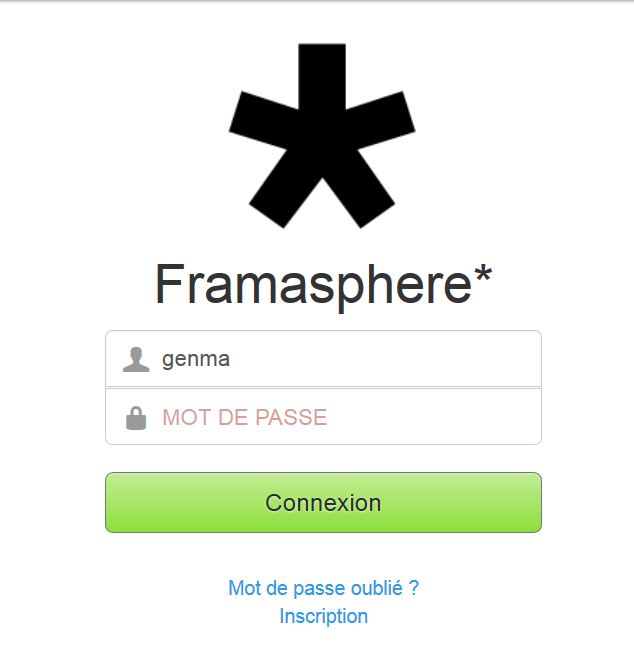
\includegraphics[scale=0.5]{./images/Framasphere.jpg}
\end{center}
\end{frame}

\begin{frame}
\begin{center}
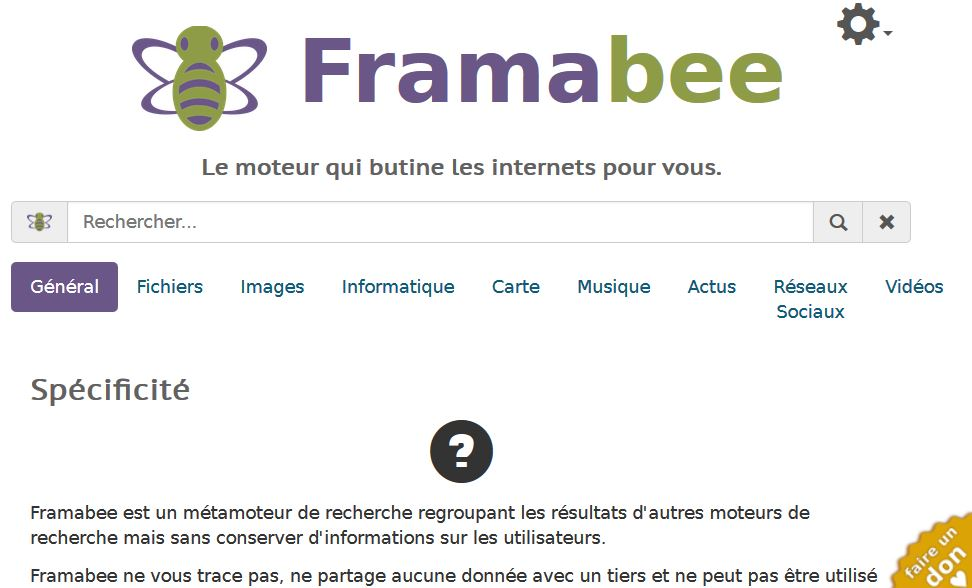
\includegraphics[scale=0.5]{./images/Framabee.jpg}
\end{center}
\end{frame}


\begin{frame}
\Huge{\centerline{Et d'autres à l'avenir...}}
\end{frame}

\begin{frame}
\begin{center}
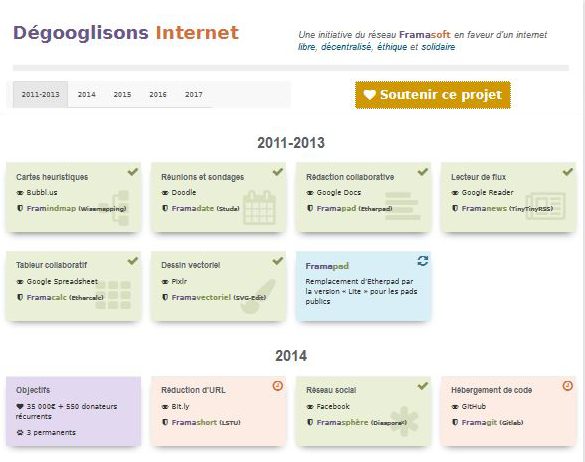
\includegraphics[scale=0.5]{./images/Roadmap.jpg}
\end{center}
\end{frame}


%----------------------------------------------------------------------------------------
\begin{frame}
\Huge{\centerline{CHATONS}}
\begin{center}
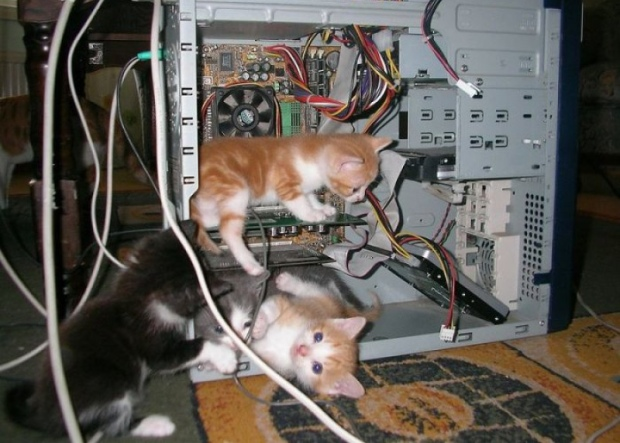
\includegraphics[scale=0.5]{./images/Cute-Kittens-In-Computer-Case.jpg}
\end{center}
\end{frame}
%------------------------------------------------

%------------------------------------------------
\begin{frame}
\frametitle{CHATONS, le collectif anti-GAFAM ?}
Collectif d'Hébergeurs Alternatifs Transparents, Ouverts, Neutres et Solidaires \url{http://chatons.org/}

\begin{block}{Le projet \emph{Dégooglisons Internet} }
Consiste à proposer des services alternatifs face à un maximum de services que nous évaluons comme menaçants pour nos vies numériques.
\justifying{
\begin{itemize}
\item Rassembler
\item  Mutualiser
\item  Décentraliser
\item Donner de la visibilité
\item Fédérer
\item  Essaimer
\item Partager
\end{itemize}
}
\end{block}
Plus de détails sur \url{http://framablog.org/2016/02/09/chatons-le-collectif-anti-gafam/}

\end{frame}

%----------------------------------------------------------------------------------------
\begin{frame}
\Huge{\centerline{Merci de votre attention.}}
\Huge{\centerline{Place aux questions. Débattons...}}
\begin{center}
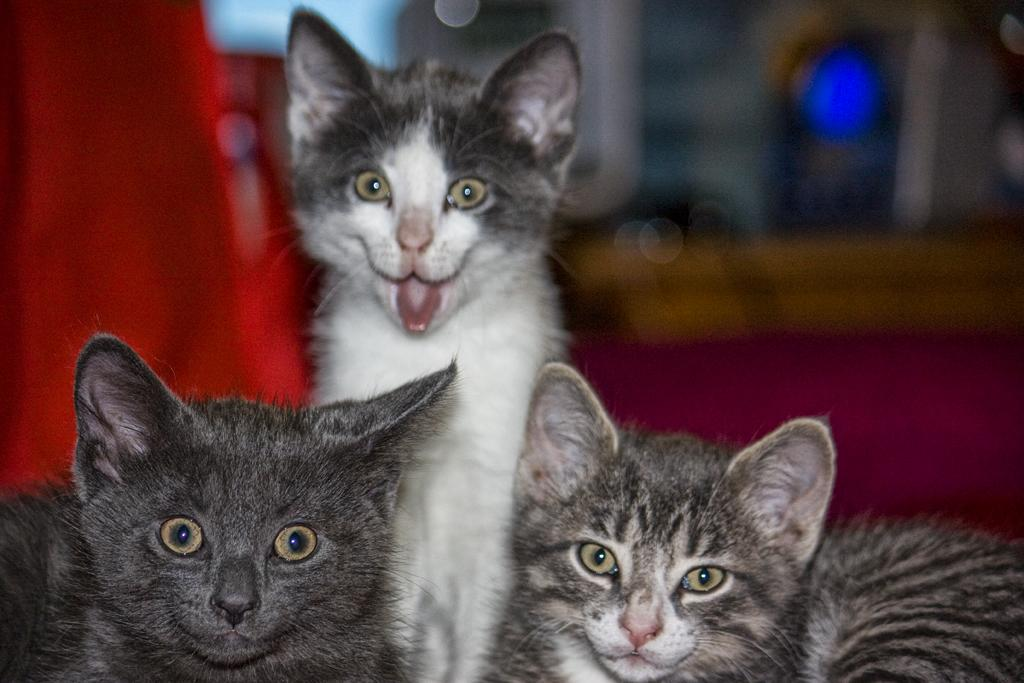
\includegraphics[scale=0.2]{./images/chat.jpg}
\end{center}
\end{frame}

%----------------------------------------------------------------------------------------
\begin{frame}
\frametitle{
\includegraphics[scale=0.4]{./images/Genma.jpg} \ \ \  A propos de moi  }
\begin{columns}[c] 

\column{.55\textwidth} 
\textbf{Où me trouver sur Internet?}
\begin{itemize}
\item Le Blog de Genma : http://genma.free.fr
\item Twitter : http://twitter.com/genma
\end{itemize}

\column{.5\textwidth} 
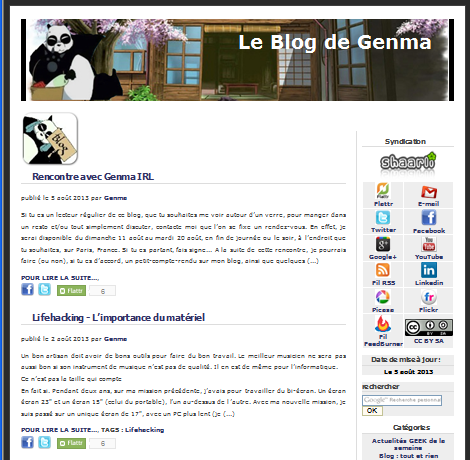
\includegraphics[width=5cm,height=5cm]{./images/blog.png} 
\end{columns}
\end{frame}


%-----------------------------------------------
\begin{frame}
\begin{center}
\Huge{Liste des services libres}
\end{center}
\end{frame}

%----------------------------------------------------------------------------------------
\begin{frame}
\frametitle{Les fonctionnalités existantes  1/2}
\begin{itemize}
\justifying{
\item \textbf{Framindmap} basé sur Wisemapping pour vos mind mapping (organisation d'idées)
\item \textbf{Framadate} basé sur Doodle qui permet de convenir d'un rendez-vous / réunion
\item \textbf{Framapad} basé sur Etherpad Lite pour éditer des documents à plusieurs
\item \textbf{Framanews} basé sur TinyTinyRSS pour suivre vos flux RSS
\item \textbf{Framacalc} basé sur Ethercalc pour éditer à plusieurs vos tableaux
\item \textbf{Framavectoriel} basé sur SVG-Edit pour créer vos images vectorielles
\item \textbf{Framasphère} basé sur Diaspora pour remplacer Facebook
\item \textbf{Framabag} basé sur Wallabag pour remplacer Pocket
\item \textbf{Frama.link} basé sur LSTU pour faire du raccourcissement d'URL
}
\end{itemize}
\end{frame}

\begin{frame}
\frametitle{Les fonctionnalités existantes 2/2}
\begin{itemize}
\justifying{
\item \textbf{Framadrive} basé sur Owncloud pour faire de l'hébergement de fichiers (et remplacer Google Drive, Dropbox...etc)
\item \textbf{Framagit} basé sur Gitlab et destiné à remplacer des hébergeurs de code comme Github
\item \textbf{Framabookin} basé sur BicBucStriim et destiné à remplacer les Google Books and co
\item \textbf{Framabee} basé sur un Searx et qui permet de faire des recherches sur le web
\item \textbf{Framapic} basé sur Lut.im qui permet d'héberger ses images
\item \textbf{Framabin} basé sur Zerobin qui permet de partager des bouts de textes comme sur Pastebin
\item \textbf{Framaboard} basé sur Kanboard qui permet de faire de la gestion de projets
\item \textbf{Framagames} pour les joueurs qui aiment les petits jeux libres
\item \textbf{Framatube} basé sur Mediagoblin pour partager des vidéos en ligne
}
\end{itemize}
\end{frame}
%----------------------------------------------------------------------------------------
\begin{frame}
\frametitle{Les prochaines fonctionnalités 1/2}
\begin{itemize}
\justifying{
\item \textbf{Framapétition} basé sur un Drupal avec WebForm pour lancer des pétitions
\item \textbf{Framatalk} basé sur Jitsi Meet qui vous permettra de discuter avec vos pôtes
\item \textbf{Framadrop} qui sort ce vendredi, basé sur LUFI qui permet de faire de l'hébergement temporaire de fichiers comme WeTransfer
\item \textbf{Framasites} basé sur PluXML pour héberger votre site web
\item \textbf{Framagenda} basé sur Webcalendar pour faire de l'agenda partagé
\item \textbf{Framacarte} basé sur uMap pour remplacer les Google Maps and co
\item \textbf{Framaslides} basé sur Strut.io pour faire des diaporamas
\item \textbf{Framameet} basé sur WanaWana pour organiser des évéments
\item \textbf{Framaloomio} basé sur Loomio pour faire de la prise de décisions
}
\end{itemize}
\end{frame}

%----------------------------------------------------------------------------------------
\begin{frame}
\frametitle{Les prochaines fonctionnalités 2/2}
\begin{itemize}
\justifying{
\item \textbf{Framatweet} basé sur Twister afin de remplacer tout ce qui est microblogging (Twitter)
\item \textbf{Frama-???} basé sur Scrumblr pour organiser ses idées
\item \textbf{Frama-???} basé sur WebODF ou PDFy pour faire du partage de PDF et remplacer des services comme Scribd
\item \textbf{Framapoulpe} basé sur Pootle pour organiser de la traduction de logiciels
\item \textbf{Framanotes} basé sur Laverna pour faire de la prise de notes comme sur Evernote
\item \textbf{Framamail} basé sur Caliopen pour héberger vos emails
\item \textbf{Framaforms} basé sur Drupal avec WebForm pour créer des questionnaires / formulaires en ligne
\item \textbf{Framalistes} basé sur Sympa pour faire de la liste de diffusion
\item \textbf{Frama-???} basé sur JsBin pour partager du code et le debugguer à plusieurs
}
\end{itemize}
\end{frame}
%----------------------------------------------------------------------------------------
\end{document}
